\section{Spécifications Techniques}


\subsection{Évaluation comparative des technologies.}
\begin{frame}{Choix pour API Gateway}
    \begin{figure}[H]
        \centering
        \begin{minipage}{0.32\textwidth}
            \centering
            
\includegraphics[height=3cm]{assets/images/spring.png}
        \end{minipage}%
        \hspace{0.03\textwidth}
        \begin{minipage}{0.32\textwidth}
            \centering
            
\includegraphics[height=3cm]{assets/images/laravel.png}
        \end{minipage}%
        \hspace{0.03\textwidth}
        \begin{minipage}{0.32\textwidth}
            \centering
            
\includegraphics[height=3cm]{assets/images/django.png}
        \end{minipage}
    \end{figure}
\end{frame}
\begin{frame}{Design Patterns - Spring}
    \begin{itemize}
        \item \textbf{Singleton Pattern} - Gestion unique des instances de services
        \item \textbf{Factory Pattern} - Création d'objets et instanciation des modèles IA
        \item \textbf{Proxy Pattern} - Contrôle d'accès et mise en cache avec Redis
        \item \textbf{Template Method Pattern} - Structure commune pour les services
        \item \textbf{Dependency Injection (DI) Pattern} - Gestion des dépendances dans Spring et FastAPI
        \item \textbf{Observer Pattern} - Communication asynchrone entre microservices
        \item \textbf{MVC (Model-View-Controller) Pattern} - Architecture Next.js et FastAPI
        \item \textbf{IoC (Inversion of Control) Pattern} - Contrôle inversé des dépendances
    \end{itemize}
\end{frame}
\begin{frame}{Benchmark Fronted}
    \begin{figure}[H]
        \centering
        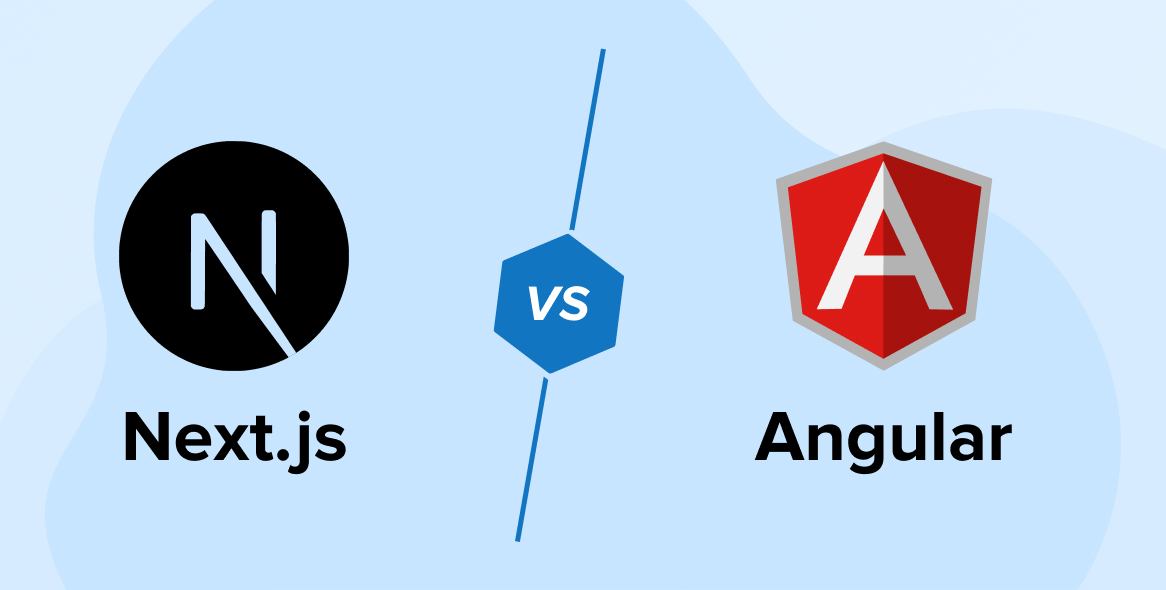
\includegraphics[height=5cm]{assets/images/bench-next.jpg}
    \end{figure}
\end{frame}

\begin{frame}{Benchmark model IA}
    \begin{figure}[H]
        \centering
        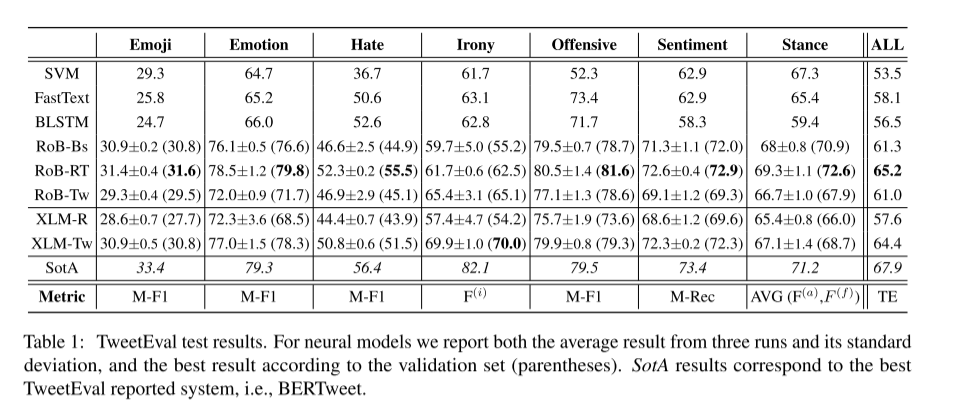
\includegraphics[height=6cm]{assets/images/ai-acc-dataset.png}
    \end{figure}
\end{frame}

\subsection{Technologies Sélectionnées}
\begin{frame}{Technologies choisies pour les services Web}
    \begin{figure}[H]
        \centering
        \begin{minipage}{0.32\textwidth}
            \centering
            
\includegraphics[height=3cm]{assets/images/next.png}
        \end{minipage}%
        \hspace{0.03\textwidth}
        \begin{minipage}{0.32\textwidth}
            \centering
            
\includegraphics[height=3cm]{assets/images/spring.png}
        \end{minipage}%
        \hspace{0.03\textwidth}
        \begin{minipage}{0.32\textwidth}
            \centering
            
\includegraphics[height=3cm]{assets/images/keycloak.png}
        \end{minipage}

    \end{figure}
\end{frame}



\begin{frame}{Technologies choisies pour IA}
    \begin{figure}[H]
        \centering

       
            
\includegraphics[height=4cm]{assets/images/ai-name.png}
    
      
    \end{figure}
\end{frame}

\begin{frame}{Technologies choisies pour Base de données et Cache}
    \begin{figure}[H]
        \centering
        \begin{minipage}{0.3\textwidth}
            \centering
            
\includegraphics[height=3cm]{assets/images/postgres.png}
        \end{minipage}%
        \hspace{0.05\textwidth}
        \begin{minipage}{0.3\textwidth}
            \centering
            
\includegraphics[height=3cm]{assets/images/redis.png}
        \end{minipage}%
        \hspace{0.05\textwidth}
        \begin{minipage}{0.3\textwidth}
            \centering
            
\includegraphics[height=3cm]{assets/images/selenium.png}
        \end{minipage}
    \end{figure}
\end{frame}
\subsection{Communication entre services}
\begin{frame}{Communication entre services}
    \begin{figure}[H]
        \centering
        
\includegraphics[height=2cm]{assets/images/rest.png}
        \hspace{0.1\textwidth}
        
\includegraphics[height=2cm]{assets/images/docker.png}
    \end{figure}
\end{frame}

\subsection{Architecture attendue}
\begin{frame}{Architecture attendue}
    \begin{figure}[H]
        \centering
        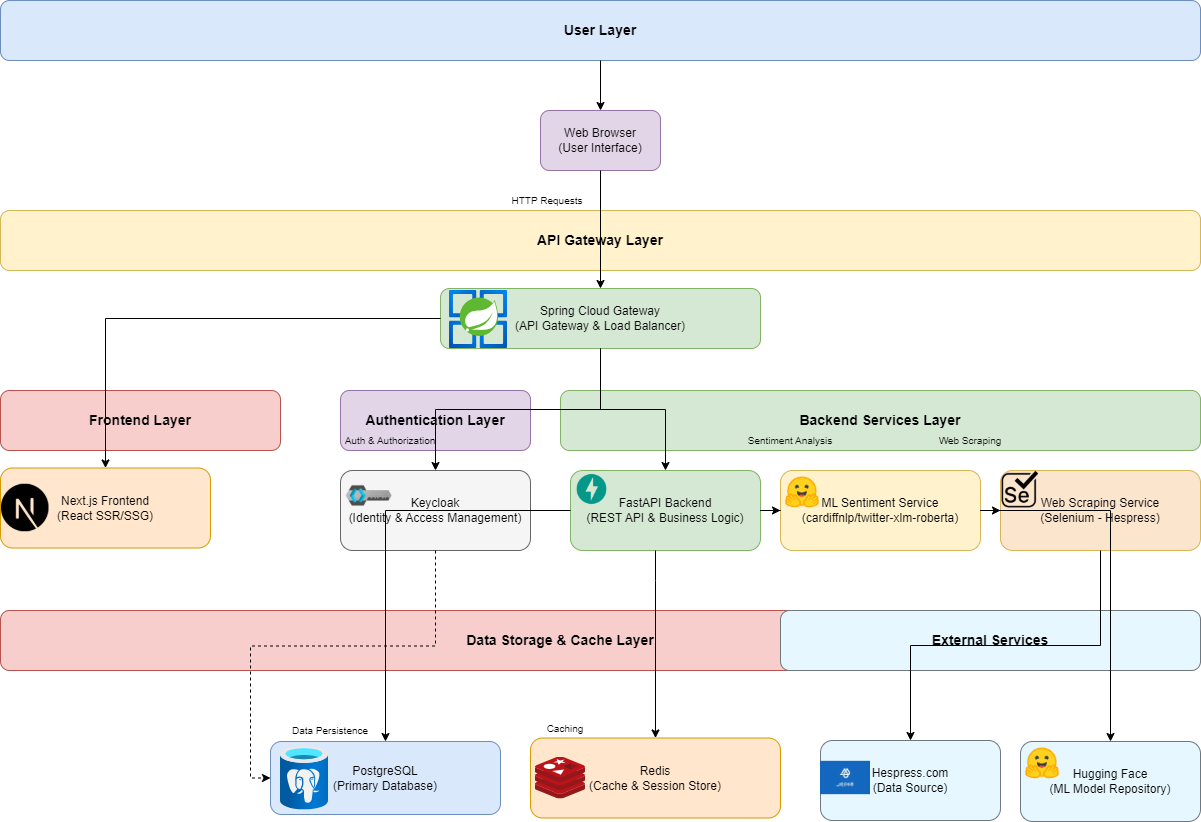
\includegraphics[height=6cm]{assets/images/arch.png}
    \end{figure}
\end{frame}

\subsection{Conclusion}
\begin{frame}{Conclusion}

    En bref, notre application de classification de sentiments des commentaires Hespress utilise une architecture microservices avec Next.js (front), FastAPI (back), Spring (API Gateway), Keycloak (auth), PostgreSQL, Redis (cache), Selenium (scraping) et le modèle cardiffnlp/twitter-xlm-roberta-base-sentiment. Ce projet a été réalisé durant mon stage au centre de formation Code 212.
\end{frame}
